
\chapter{KẾT QUẢ VÀ ĐÁNH GIÁ}
\label{chap:evalution}

\section{Phương pháp đánh giá}

Quá trình đánh giá được thực hiện qua hai độ đo chính là: Mean Opinion Scores (MOS) và Fréchet Inception Distance (FID).

\subsection{Đánh giá dựa trên cảm nhận của con người}

\subsubsection{Mean Opinion Scores (MOS)}

Hiện tại, chưa có một độ đo chung cho bài toán sinh cử chỉ, đặc biệt là sinh cử chỉ từ giọng nói, vì vậy luận văn dựa vào đánh giá chủ quan của con người để thực hiện các đánh giá thực nghiệm. 
Tương tự như các phương pháp trước đây \cite{yoon2022genea}, \cite{kucherenko2021large}, các mô hình sinh cử chỉ điều khiển bằng giọng nói vẫn thiếu các chỉ số mục tiêu phản ánh một cách nhất quán với nhận thức chủ quan của con người  \cite{alexanderson2022listen}.

MOS được đo lường thông qua ba tiêu chí:

\begin{itemize}
	\item Human-likeness (Mức độ giống con người)
	\item Gesture-Speech Appropriateness (Sự phù hợp giữa cử chỉ và giọng nói)
	\item Gesture-style Appropriateness (Sự phù hợp giữa phong cách cử chỉ)
\end{itemize}

Một trong những đóng góp của luận văn là xây dựng  \hyperlink{https://genea-workshop.github.io/leaderboard/}{GENEA Leaderboard} \footnote{  \url{https://genea-workshop.github.io/leaderboard} } \cite{nagy2024towards}. Hệ thống này bao gồm HEMVIP (\textbf{H}uman \textbf{E}valuation of \textbf{M}ultiple \textbf{V}ideos in \textbf{P}arallel) nhằm so sánh kết quả sinh trực quan giữa các video được tạo ra từ kết quả kết xuất.

\begin{figure}[H]
	\centering
	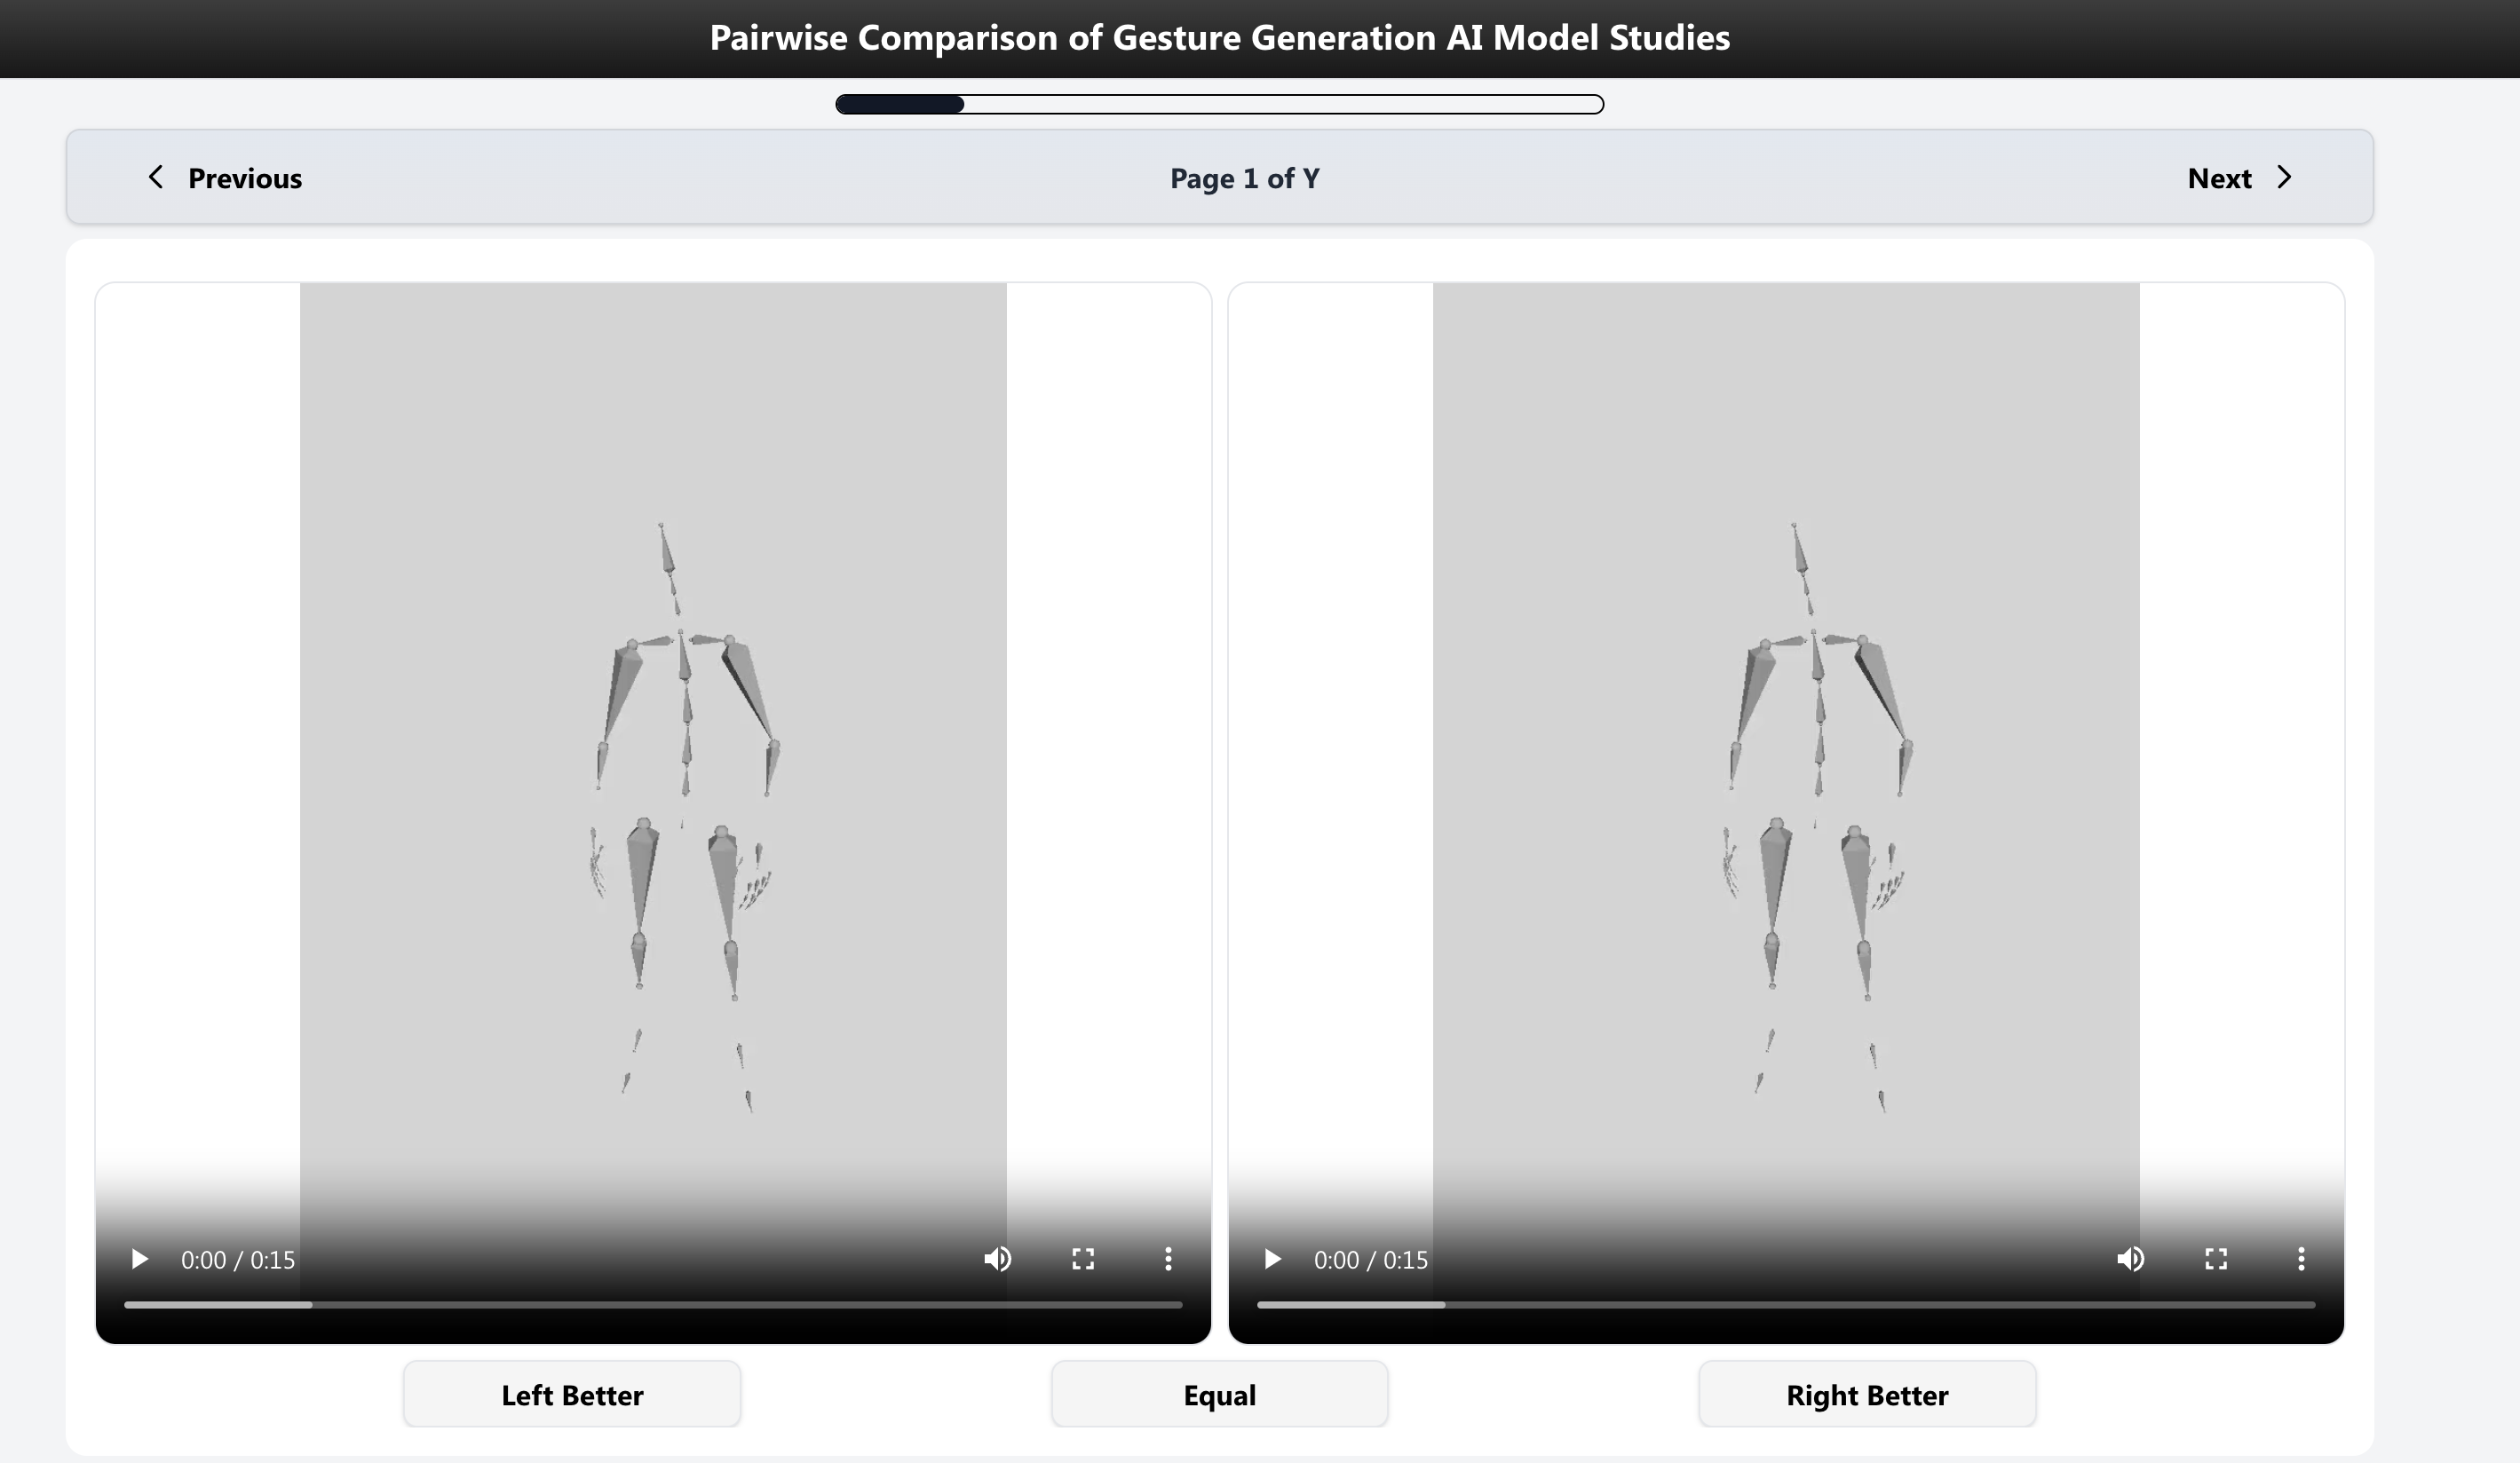
\includegraphics[width=\textwidth]{hemvip}
	\caption{Hệ thống HEMVIP nhằm đánh giá kết quả sau khi kết xuất của hai mô hình}
\end{figure}

Trong nhóm GENEA (\textbf{G}eneration and \textbf{E}valuation of \textbf{N}on-verbal Behaviour for \textbf{E}mbodied \textbf{A}gents), chúng tôi sẽ thuê các người đánh giá trên Prolific và thực hiện nghiên cứu người dùng (User Study) theo kết quả kết xuất trên video, người tham gia sẽ đánh giá \textit{Bên Trái Tốt Hơn} (Left Better), \textit{Bằng Nhau} hoặc \textit{Bên Phải Tốt Hơn} (Right Better). Điểm số sẽ cập nhật sẽ là $-1$, $0$ và $1$ cho mô hình cho các kết quả sinh bao gồm cả dữ liệu thật. Kết quả so sánh của toán bộ mô hình sẽ được cập nhật bằng hệ thống đánh giá Elo (Elo rating system).

Mã nguồn của chương trình được công khai ở \hyperlink{https://github.com/hemvip/hemvip.github.io/}{github.com/hemvip.github.io}
\footnote{HEMVIP 2 \url{https://github.com/hemvip/hemvip.github.io}}.


\subsection{Đánh giá dựa trên các độ đo số học}

\subsubsection{Sai số toàn phương trung bình (Mean Square Error)}

Độ đo sai số toàn phương trung bình giữa chuỗi cử chỉ dự đoán $\hat{\mathbf{y}}_i^{1:M \times D}$ và chuỗi cử chỉ thật $\mathbf{y}_i^{1:M \times D}$ được thực hiện theo công thức sau:

\begin{equation}
\text{MSE} = \frac{1}{n} \sum_{i=1}^n \left\| \mathbf{y}_i^{1:M \times D} - \hat{\mathbf{y}}_i^{1:M \times D} \right\|^2
\end{equation}

Trong đó:  
\begin{itemize}
	\item $n$ là số lượng mẫu dữ liệu.
	\item $\mathbf{y}_i^{1:M \times D}$ là giá trị thực (ground truth) của mẫu thứ $i$, với $M$ là số khung (frames) và $D$ là số chiều dữ liệu.
	\item $\hat{\mathbf{y}}_i^{1:M \times D}$ là giá trị dự đoán của mẫu thứ $i$, có cùng kích thước $M \times D$.
	\item $\left\| \mathbf{y}_i^{1:M \times D} - \hat{\mathbf{y}}_i^{1:M \times D} \right\|^2$ là bình phương chuẩn của sự chênh lệch giữa ma trận thực và ma trận dự đoán.
\end{itemize}

MSE đo lường độ chênh lệch trung bình bình phương giữa các chuỗi cử chỉ thực và chuỗi cử chỉ dự đoán, càng nhỏ thì mô hình dự đoán càng chính xác. Kết quả đánh giá được cập nhật ở \autoref{subsec:MSEResult}.

\subsubsection{Fréchet Gesture Distance (FGD)}

Tương tự các phương pháp sinh ảnh sử dụng độ đo FID (Fréchet Inception Distance) nhằm đo khoảng cách phân phối của dữ liệu thật và dữ liệu dự đoán.
Khoảng cách Fréchet trong cử chỉ hay FGD (\textbf{F}réchet \textbf{G}esture \textbf{D}istance) đo sự tương đồng về phân phối giữa chuỗi cử chỉ sinh ra $\hat{\mathbf{y}}_i^{1:M \times D}$ và cử chỉ thực tế  $\mathbf{y}_i^{1:M \times D}$:

\begin{equation}
	\text{FGD} = \left\| \hat{\mu} - \mu \right\|^2 + \operatorname{Tr}\left( \Sigma + \hat{\Sigma} - 2 \sqrt{\Sigma \hat{\Sigma}} \right)
	\label{eq:fidscore}
\end{equation}

Trong đó trong đó $n$ là số lượng mẫu dữ liệu, các tham số:

\begin{itemize}
	\item $\mu = \frac{1}{n} \sum_{i=1}^n \mathbf{y}_i^{1:M \times D}$ và $\hat{\mu} = \frac{1}{n} \sum_{i=1}^n \hat{\mathbf{y}}_i^{1:M \times D}$ lần lượt là vector trung bình của các đặc trưng (features) từ tập dữ liệu thực $\mathbf{y}_i^{1:M \times D}$ và tập dữ liệu sinh $\hat{\mathbf{y}}_i^{1:M \times D}$.
	 
	\item $\Sigma = \frac{1}{n-1} \sum_{i=1}^n \left( \mathbf{y}_i^{1:M \times D} - \mu \right) \left( \mathbf{y}_i^{1:M \times D} - \mu \right)^T$ và
	
	$\hat{\Sigma} = \frac{1}{n-1} \sum_{i=1}^n \left( \hat{\mathbf{y}}_i^{1:M \times D} - \hat{\mu} \right) \left( \hat{\mathbf{y}}_i^{1:M \times D} - \hat{\mu} \right)^T$: là ma trận hiệp phương sai (covariance matrix) của các đặc trưng từ tập dữ liệu thực và sinh.
	
	\item $\operatorname{Tr}(\cdot)$ là toán tử vết (trace) của ma trận, tính tổng các phần tử trên đường chéo chính.
	
	\item $\sqrt{\Sigma \hat{\Sigma}}$: là căn bậc hai ma trận (matrix square root) của tích hai ma trận hiệp phương sai.
\end{itemize}

FGD thấp cho thấy phân phối của cử chỉ sinh ra gần giống với cử chỉ thực tế, trong khi FID cao gợi ý sự khác biệt lớn, cho thấy chất lượng cử chỉ sinh ra kém hơn. Trong luận văn, quá trình đánh giá được thực hiện trên chuỗi cử chỉ dự đoán $\hat{\mathbf{x}}^{0} \in \mathbb{R}^{1:M \times D}$ và chuỗi cử chỉ thật $\mathbf{x}_{0} \in \mathbb{R}^{1:M \times D}$.


\section{Kết quả đánh giá}
\label{sec:result}

\subsection{Kết quả đánh giá nghiên cứu người dùng}

\subsubsection{Kết quả đánh giá bằng MOS}

Ở đây luận văn sử dụng lại kết quả đánh giá của mô hình baseline \textbf{DiffuseStyleGesture} \cite{yang2023diffusestylegesture} trong độ đo về  cảm nhận đánh giá của con người do lĩnh vực sinh cử chỉ vẫn còn rất mới, chi phí để ước lượng các mô hình còn lớn nên luận văn không thể đánh giá được mô hình OHGesture. Vì vậy các kết quả này chưa bao gồm thông tin kết quả về mô hình \textbf{OHGesture} mà luận văn đề xuất.

\begin{figure}[htbp]
	\centering
	\begin{subfigure}[b]{0.3\textwidth}
		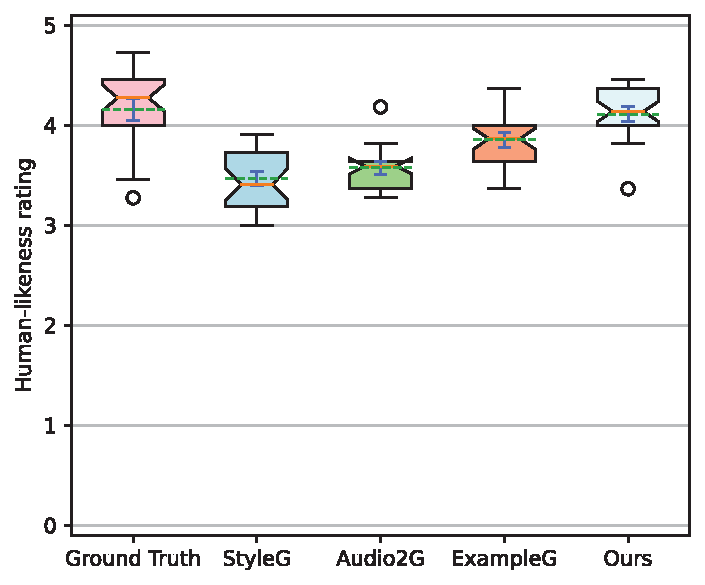
\includegraphics[width=\textwidth]{BoxHumanLikeness.pdf}
		\caption*{(a) Human-likeness}
	\end{subfigure}
	\hfill
	\begin{subfigure}[b]{0.3\textwidth}
		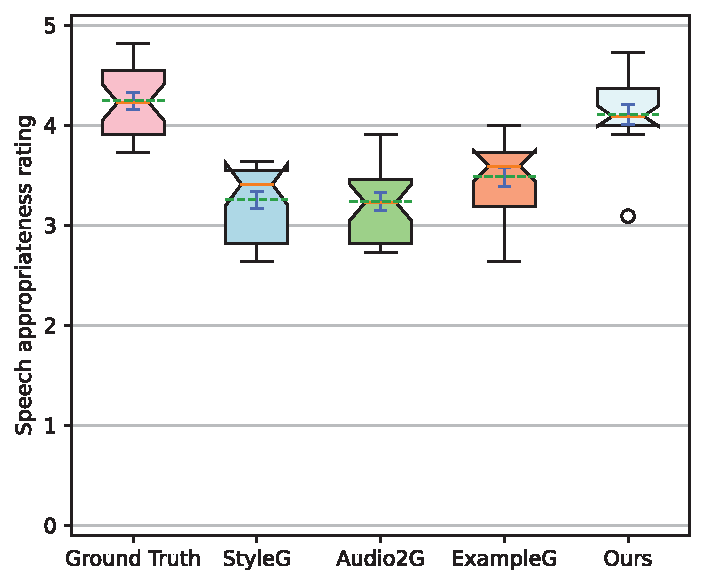
\includegraphics[width=\textwidth]{BoxSpeechAppropriateness.pdf}
		\caption*{\small (b) Speech Appropriateness}
	\end{subfigure}
	\hfill
	\begin{subfigure}[b]{0.3\textwidth}
		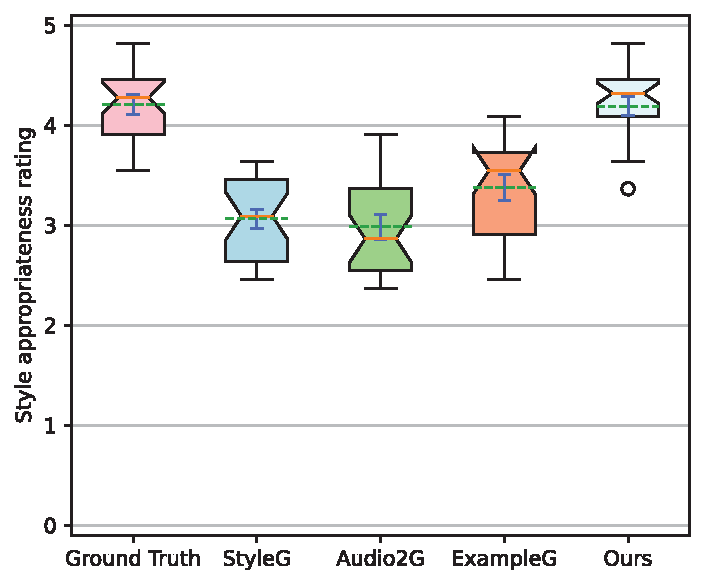
\includegraphics[width=\textwidth]{BoxStyleAppropriateness.pdf}
		\caption*{(c) Style Appropriateness}
	\end{subfigure}
	
	\label{fig:compare }
\end{figure}


Để hiểu hiệu suất thị giác thực tế của phương pháp của luận văn, luận văn tiến hành một nghiên cứu người dùng so sánh các cử chỉ được tạo ra từ phương pháp của luận văn và dữ liệu chụp chuyển động thực tế. Độ dài của các đoạn clip đánh giá dao động từ 11 đến 51 giây, với độ dài trung bình là 31.6 giây, dài hơn so với các đoạn trong đánh giá GENEA \cite{yoon2022genea} (8-10 giây), vì thời gian dài hơn có thể tạo ra kết quả rõ ràng và thuyết phục hơn \cite{yang2022reprgesture}. Người tham gia đánh giá trên thang điểm từ 5 đến 1, với các nhãn từ $\texttt{excellent}$,  $\texttt{good}$, $\texttt{fair}$, $\texttt{poor}$, đến $\texttt{bad}$. 

\begin{table}[H]
	\centering
	\begin{tabular}{lcc}
		\hline
		\multicolumn{1}{c}{Name} &
		\begin{tabular}[c]{@{}c@{}}Human\\ likeness \end{tabular}$\uparrow$ &
		\begin{tabular}[c]{@{}c@{}}Gesture-speech\\ appropriateness\end{tabular}$\uparrow$ \\ \hline
		Ground Truth          & 4.15 $\pm$ 0.11          & 4.25 $\pm$ 0.09          \\
		Ours                  & \textbf{4.11 $\pm$ 0.08} & \textbf{4.11 $\pm$ 0.10} \\
		\quad$-$ WavLM             & 4.05 $\pm$ 0.10          & 3.91 $\pm$ 0.11          \\
		\quad$-$ Cross-local attention   & 3.76 $\pm$ 0.09          & 3.51 $\pm$ 0.15          \\
		\quad$-$ Self-attention    & 3.55 $\pm$ 0.13          & 3.08 $\pm$ 0.10          \\
		\quad$-$ Attention + GRU&
		3.10 $\pm$ 0.11 &
		2.98 $\pm$ 0.14 \\
		\quad$+$ Forward attention & 3.75 $\pm$ 0.15          & 3.23 $\pm$ 0.24          \\
		\hline
	\end{tabular}
	\caption{Kết quả đánh giá bằng MOS}
	\label{table:MOSScore}
\end{table}
%Kết quả của các nghiên cứu loại bỏ (Ablation studies). "$-$" chỉ các mô-đun không được sử dụng và "$+$" chỉ các mô-đun bổ sung. Chữ in đậm chỉ ra chỉ số tốt nhất

\subsection{Kết quả đánh giá theo độ đo số học}

\subsubsection{Kết quả đánh giá bằng MSE}
\label{subsec:MSEResult}

Trong luận văn, chuỗi cử chỉ dự đoán sẽ được đoạn trên $M$ khung hình. Luận văn sử dụng Mean Square Error trên chuỗi cử chỉ $\mathbf{x}^{1:M \times D}$.

\begin{table}[H]
	\centering
	\resizebox{\textwidth}{!}{%
		\begin{tabular}{lcccccc}
			\hline
			\multicolumn{1}{c}{Cảm xúc} & Tự Nhiên & Buồn Bã &  Vui Vẻ  & Thư Giãn & Lớn Tuổi & Giận Dữ \\ \hline
			DiffuseStyleGesture  & 75.04 & 51.40 & 110.18 & 130.83     & 116.03    & 78.53     \\
			ZeroEGG & 136.33 & 81.22 & 290.47 & 140.24     & 102.44    & 181.07     \\
			\hline
			Mô hình đề xuất                     &         &         &         &           &          &                 \\
			\quad \textbf{OHGesture} & 161.22 & 89.58 & 279.95 & 156.93   & 99.86   & 215.24    \\
			\hline
		\end{tabular}%
	}
	\caption{Kết quả đánh giá Mean Square Error theo 6 cảm xúc}
	\label{table:EvaluationMSE}
\end{table}


\subsubsection{Kết quả đánh giá bằng FGD}

Luận văn đề xuất Fréchet Gesture Distance (FGD), độ đo FID dựa trên cử chỉ (gesture), và xây dựng mã nguồn \hyperlink{https://github.com/GestureScore/GestureScore}{GestureScore} \footnote{Github/GestureScore: \url{https://github.com/GestureScore/GestureScore}} . Trong GestureScore, luận văn xây dựng một Inception V3 model, để mã hóa chuỗi khung hình $\bx^{1:M \times D}$ thành vector tiềm ẩn kích thước $32 \times 32$. Sử dụng vector này làm đầu vào cho \autoref{eq:fidscore}. Sau đây là \autoref{table:EvalFGD} đánh giá kết quả của mô hình OHGesture bằng GestureScore

%$\uparrow$
\begin{table}[H]
	\centering
	\begin{tabular}{lcc}
		\hline
		\multicolumn{1}{c}{Name} & FGD trên vector đặc trưng & \begin{tabular}[c]{@{}c@{}} FGD dữ liệu gốc \end{tabular} \\ \hline
		Ground Truth             & -       & -          \\
		Ours                     &       & \\
		\quad OHGesture (Feature D=1141) & 2.058      & 9465.546 \\
		\quad OHGesture (Rotations) & 3.513       & 9519.129 \\
		\hline
	\end{tabular}
	\caption{Kết quả đánh giá Fréchet Gesture Distance (FGD) trên $\bx^{1:M \times D}$ (từ khung hình 1 đến khung hình M, mỗi khung hình có D đặc trưng từng khung hình )}
		\label{table:EvalFGD}
\end{table}

\begin{itemize}[]
		\item \textbf{Vector đặc trưng}
	Sử dụng tệp BVH để chuyển toàn bộ skeleton của mỗi khung hình thành vector đặc trưng $D = 1141 $ như công thức  \autoref{eq:gesturevector}
	
	\item  \textbf{Rotations}: Từ tệp BVH kết quả, luận văn trích xuất sự thay đổi của các góc quay (rotations), $D = 225$ ($225 = 75 \times 3$) của chuỗi cử chỉ với chiều dài mỗi đoạn là $M$ khung hình để đánh giá ở dòng OHGesture bên dưới. 
	
\end{itemize}

\section{Xây dựng và tiêu chuẩn hóa hệ thống đánh giá kết quả sinh cử chỉ}

Hiện nay các mô hình sinh (gesture generation) cử chỉ được quan tâm nghiên cứu với rất nhiều mô hình khác nhau, tuy nhiên do không có độ đo chung, vì các độ đo truyền thống như FID (Fréchet Inception Distance) hay IS (Inception Score),.. không thể hiện được hết các tính chất Giống người (Human-likeness), tính phù hợp với giọng nói (Speech Appropriateness), và tính phù hợp với phong cách (Style Appropriateness) của cử chỉ. Các mô hình cũng được thực hiện và huấn luyện trên một tập dữ liệu khác nhau, vì vậy rất khó để biết được mô hình nào đã đạt kết quả tốt hơn, và mô hình nào là mô hình state-of-the-art, từ đó khó có thể đạt được sự tiến bộ trong lĩnh vực sinh cử chỉ. Việc thiếu tiêu chuẩn chung để đánh giá trong cộng đồng nghiên cứu khiến luận văn mong muốn xây dựng một hệ thống xếp hạng trực tuyến \cite{nagy2024towards} \hyperlink{https://genea-workshop.github.io/leaderboard/}{GENEA Leaderboard} \footnote{GENEA Leaderboard: \url{https://genea-workshop.github.io/leaderboard/}}, là một bảng xếp hạng các mô hình sinh cử chỉ. Luận văn thu thập và xử lý một tập dữ liệu cử chỉ từ nhiều ngôn ngữ và từ nhiều tập dữ liệu khác nhau và tiêu chuẩn hóa để tạo ra một tập dữ liệu duy nhất.  Sau đó, luận văn sẽ mời các tác giả của các mô hình để học và dự đoán trên tập dữ liệu đã được tiêu chuẩn hóa, sau khi có kết quả sinh cử chỉ, luận văn sẽ thuê những người tham gia nghiên cứu trên Prolific để đánh giá và xếp hạng kết quả sinh cử chỉ của các mô hình. Hiện tại luận văn đang xây dựng hệ thống trực tuyến \hyperlink{https://github.com/hemvip/hemvip.github.io}{hemvip/hemvip.github.io}\footnote{HEMVIP2 \url{https://github.com/hemvip/hemvip.github.io}} với mục tiêu đánh giá kết quả sinh của cử chỉ thông qua việc thuê các người tham gia đánh giá kết quả thông qua Prolific. Luận văn sẽ bổ sung các đánh giá về mô hình OHGesture dựa trên các điểm số trên.


Thông qua hệ thống đánh giá này, nghiên cứu kỳ vọng sẽ thiết lập một tiêu chuẩn chung, từ đó tạo động lực cho sự tiến bộ trong lĩnh vực sinh cử chỉ.
